%\chapter{3HDM}
%\label{ch:3HDM}

\newpage 

\chapter{Proper 3HDM }

%\section{Not used yet}

%We used previous work to narrow down the vast parameter space of these type of models offer, see \cite{Ferreira_2018,Ivanov_2012,Ivanov_2016,Aranda_2017}.
%
%Our conclusions are consistent with these studies, where it was found to have large regions of parameter space which conformed with experimental constraints in the flavour and scalar sectors.

\section{Introduction}

Now having finished the analysis of a simple unitary extension, it is time to present a more complex model. 
%
The goal of this chapter will be to first introduce all the required theoretical background to analysis a three Higgs Doublet Model (3HDM), specifically a minimal BGL (Branco-Grimus-Lavoura) like 3HDM. 
% 
Then moving to present a phenomenological simulation similar as before, as to observe the state of the art in the 3HDM. 
%
This simulation used a newer version of the previously discussed mechanism with the addition of a flavour calculation package based on python3 entitled "flavio" { \color{blue} citation needed}  

This 3HDM model is part of a larger family of multiple Higgs Doublet Models, or NHDMs, the first iteration of which was the 2HDM model. 
% 
As before mentioned, one of the simplest ways to expand the SM is to add elements to it's scalar sectors. 
%
In these types of models, in parallel with the standard SM Higgs doublet some additional replicas of that same doublet are introduced. 
%
In the 3HDM these form a sort of family in the scalar sector in analogy to the fermion sector. 
%
This idea is far from original and was first discussed by Weinberg in, \cite{Weinberg1976}.

These additional Higgs doublet are valid given they do not alter the tree-level electroweak $\rho$ parameter as long the condition that the sum of the doublet VEVs are equal the value for the electroweak VEV in case of the SM {\color{blue} citation needed}. 
% 
Although this value can vary by 20\% { \color{blue} citation needed} there are many reason as to impose this condition.
%
This is the part of a wider \textit{alignment limit} condition that will be discussed further on, in depth. { \color{blue} True? } 

The basis for our BGL like treatment of a 3HDM will be the inclusion of a flavour symmetry, as to attempt to constrain the flavour observables. In particular the addition of a $\mathrm{U}(1) \times \mathrm{Z}_2$ symmetry.
% 
This symmetry constrains the terms that can appear in the flavour sector of the Lagrangian resulting in very specific structures (or textures) of the Yukawa couplings.
% 
We will show how this structure combined with the off diagonal terms of the CKM matrix lead to controlled values for FCNCs. 
%
% achieving a similar mechanism to that of the BGL 2HDM. 
%
Then showing that light scalars are still within the reach of future collider experiments in our model's framework while having FCNCs concurrent with observations and respecting many more theoretical and experimental bounds, such as in our previous analysis. 


\subsection{Context, the case of the BGL-2HDM}

The first model that attempted to perform a doublet based extension was the Two Higgs Doublet Model (2HDM) proposed by T.D. Lee \cite{Lee1973}.  
%
His work motivated by the search for a spontaneous breaking of the CP symmetry. 

A great deal of interest was invested in 2HDMs, given their possible dark matter candidates large particle spectrum, including charged and additional neutral scalars.
%
However, take in consideration that in most 2HDM structures the possibility of tree-level scalar mediated FCNCs emerged. 
% 
A analysis of their origin led to disturbing conclusions, given the fermions now have their mass generated by several Yukawa matrices their simultaneous diagonalization wasn't guaranteed. 
%
These tree-level FCNCs are, in most cases, in direct opposition to experimental results, as discussed in Chapter 1. 
%
In fact, Consulting the literature, as in, \cite{Branco:1999fs}, we see that this forces the extra scalars in the 2HDM case to have masses above 1 TeV.
%
These heavy scalars although a possibility given current observations, are far from ideal, since there is no indication such heavy scalars exist nor do they provide us with interesting physics. 
%
There-for several mechanisms have been proposed to deal with suppress these tree-level FCNCs as to allow for richer physics. 
%
First, in, \cite{Ferreira_2011,Nebot_2015,ferreira2019strong}, it is proposed a framework in which we have the balancing of CP-odd and CP-even contribution to FCNCs, however, this would requires some fine-tuning, making it very unappealing. 
% 
Another possibility is to assume alignment between different Yukawa matrices such that no FCNCs are present, see \cite{Pich_2009,Jung_2010,Jung_2011} for more information. 
%
Finally we could also use the approach presented in the BGL version of the 2HDM \cite{Branco_1996,LAVOURA1994}, here the authors impose a flavour-violating symmetry naturally keeping the FCNCs under control trough the CKM matrix. 
%
The phenomenology of the model has been studied quite thoroughly in previous works, see Refs. \cite{Botella_2014,Botella_2016}, and it remains a possible scenario for BSM physics.
%
Inspired by this BGL model our studies will try to reproduce a similar mechanism on a 3HDM Model. 


\section{The formulation of a BGL-like 3HDM} 

Challenging the 2HDM BGL paradigm can be motivated by some phenomenological comparison of the 3HDM to the 2HDM model more than just by the "naturalist" family argument.
%
For example, vacuum stability in the 2HDM model can only accommodate one instance of spontaneous CP or charge symmetry breaking \cite{Branco_2012,Ferreira_2004,Barroso_2007}. 
%
However in Multiple Higgs Doublets models (NHDMs), such as the 3HDM, charge breaking minima were found to be stable while at the same time coexisting with charge-preserving ones, for more information see, \cite{Barroso_2006}.   
%
Also, for the 2HDM a full list of all possible incorporations of symmetries consistent with $\mathrm{SU(2)}\times\mathrm{U(1)}$ has been achieved \cite{Ivanov_2008,Ivanov2007}, while for the 3HDM no work has thus far been completed, see, \cite{Ivanov_2012,Ivanov_2015}. 
%
Moreover generic unitarity constraints have been found for the 2HDM \cite{Ginzburg_2005} but not for 3HDMs. 
%
Not to mention these models provide a richer playground for experimental detection and testing than the 2HDM give it's extended scalar sector. 

\subsection{Fields and the Additional $\mathrm{U(1)}\times\mathbb{Z}_2$ Symmetry}

In a sense this model is extension of the SM as it still includes all the same fields with same charges under the $\mathcal{G}_{SM}$ as we saw in chapter 1. 
% 
Making the particle content of the model is pretty similar to the SM. 
%
Having the same gauge fields and the following fermion and scalar fields,
%
\begin{equation}
\label{eq:3HDM_Fields}
\begin{gathered}
Q_{L_i} =  \begin{pmatrix}
u_{L_i}  \\
d_{L_i}
\end{pmatrix} \quad , \quad \Psi_{L_i} =  \begin{pmatrix}
\nu_{L_i}  \\
e_{L_i}
\end{pmatrix} \quad , \quad \\ 
u_{R_i} \quad , \quad d_{R_i} \quad , \quad e_{R_i} \quad i=\{1,2,3\} \quad ,  \\  
\phi_k = \begin{pmatrix}
W_k^\pm + i \, W_k^\mp \\ 
\frac{1}{\sqrt{2}}\left( v_k + h_k + i Z_k \right) 
\end{pmatrix}  \quad , \quad k=\{ 1,2,3\} \quad . 
\end{gathered} 
\end{equation}
%
where $Q_{L_i}$ , $\phi_k$ , $\Psi_{L_i}$ and $u_{R_i}$, $d_{R_i}$, $e_{R_i}$ are $\mathrm{SU}(2)_L$ doublets and singlets of the i-th and k-th generation, respectively. 
%
However the new charges under $\mathrm{U(1)}\times\mathbb{Z}_2$ must be specified. 
%
They show themselves in the transformation these fields can perform, 
%
\begin{equation}
\label{eq:3HDM_Transformations}
	\begin{split} 
	\mathrm{U(1)} : & \\
		& Q_{L_3} \rightarrow    e^{i \alpha} Q_{L_3}  \\  
		& u_{R_3} \rightarrow    e^{2 i \alpha} u_{R_3}  \\
		& \phi_1  \rightarrow    e^{i \alpha} \phi_1  \\   
		& \Psi_{L_1} \rightarrow e^{i \alpha} \Psi_{L_1} \\
		& \phi_3 \rightarrow     e^{i \alpha} \phi_3  \\ 
	\end{split} \quad \quad \quad  
	\begin{split}
		\mathbb{Z}_2 : & \\
		 	& Q_{L_3} \rightarrow -Q_{L_3} \\
		 	& u_{R_3} \rightarrow -u_{R_3} \\ 
		 	& \phi_1  \rightarrow -\phi_1 \\ 
		 	& \Psi_{L_1} \rightarrow - \Psi_{L_1} \\ 
		 	& \phi_3 \rightarrow -\phi_3
	\end{split} 
\end{equation} 
%
All remaining fields not shown in Eq. \ref{eq:3HDM_Transformations} remain unchanged under transformations of the $\mathrm{U(1)}\times\mathbb{Z}_2$ global symmetry (one scalar field and two fermion generations).  
%
This symmetry will have to be softly broken as to avoid the appearance of a massless Goldstone state.

Note there is no right handed neutrino fields in this model making it so that no neutrino mass terms appear. { \color{blue} check with morais } 

\subsection{Introducing The Scalar Sector}

Let us then start our proper introduction to the workings of the model by presenting the scalar sector where the new spin-0 $\mathrm{SU(2)}$ doublets, $\phi_i$, $i=\{1,2,3\}$ reside. 
\begin{comment}
The scalar doublets are made to transform under the imposed $\mathrm{U(1)}\times \mathbb{Z}_2$ symmetries as, 
%
\begin{equation}
\begin{split}
\mathrm{U(1)} & : \phi_1 \rightarrow \phi_1 e^{i \alpha} \quad ,
            \quad \phi_3 \rightarrow \phi_3 e^{i \alpha}  \\
\mathbb{Z}_2  & : \phi_1 \rightarrow -\phi_1 \ \ \quad , 
            \quad \phi_2 \rightarrow \phi_2  \quad , 
            \quad \phi_3 \rightarrow \phi_3 \quad .
\end{split}
\end{equation}
\end{comment}
Note the scalar potential to be CP-invariant, this means,
\begin{equation}
\phi_1 = \phi_1^{\**} \quad , \quad \phi_2 = \phi_2^{\**} \quad , \quad 
\phi_3 = \phi_3^{\**} 
\end{equation}
The generic scalar potential that follows all these transformations is extensively written in, 
\begin{equation}
\label{eq:3HDM_Scalar_Pot}
\begin{split}
V(\phi_i) = & 
- \mu_1^2 \left( \phi^{\dagger}_1 \phi_1 \right) 
- \mu_2^2 \left( \phi^{\dagger}_2 \phi_2 \right)  
- \mu_3^2 \left( \phi^{\dagger}_3 \phi_3 \right) \\ 
& \left[ - \mu_{12}^2 \left( \phi^{\dagger}_1 \phi_2  \right) 
  - \mu_{23}^2 \left( \phi^{\dagger}_2 \phi_3  \right)  
  - \mu_{13}^2 \left( \phi^{\dagger}_1 \phi_3  \right) + h.c. \right]  \\
& + \lambda_1 \left( \phi^{\dagger}_1 \phi_1 \right) 
  + \lambda_2 \left( \phi^{\dagger}_2 \phi_2 \right)  
  + \lambda_3 \left( \phi^{\dagger}_3 \phi_3 \right) \\  
& + \lambda_4 \left( \phi^{\dagger}_1 \phi_1 \right)  \left( \phi^{\dagger}_2 \phi_2 \right) 
  + \lambda_5 \left( \phi^{\dagger}_1 \phi_1 \right)  \left( \phi^{\dagger}_3 \phi_3 \right)  
  + \lambda_6 \left( \phi^{\dagger}_2 \phi_2 \right)  \left( \phi^{\dagger}_3 \phi_3 \right)  \\ 
& + \lambda_7 \left( \phi^{\dagger}_1 \phi_2 \right)  \left( \phi^{\dagger}_1 \phi_2 \right)  
  + \lambda_8 \left( \phi^{\dagger}_1 \phi_3 \right)  \left( \phi^{\dagger}_3 \phi_1 \right)   
  + \lambda_9 \left( \phi^{\dagger}_2 \phi_3 \right)  \left( \phi^{\dagger}_3 \phi_2 \right)  \\
& + \lambda_{10} \Bigg\{ \left( \phi^{\dagger}_1 \phi_3 \right)^2 + \text{h.c.} \Bigg\}   
\end{split} 
\end{equation}
%
Due to the $\mathcal{CP}$ symmetry imposed on this potential all parameters, $(\lambda_i,i=\{1,...,10\})$, here are real.
%
The parameter $\mu_{23}$, is necessarily added as to impede the formation of a massless axion. 
%
However the most generic version of this soft breaking is given by the second line.  
%
After the process of SBB, all Higgs doublets take a VEV shape similar to that of the SM Higgs, written as, 
%
\begin{equation}
\phi_k = 
\begin{pmatrix}
W_k^\pm + i \, W_k^\mp \\ 
\frac{1}{\sqrt{2}}\left( v_k + h_k + i Z_k \right)
\end{pmatrix}  \rightarrow \langle \phi_k \rangle = \begin{pmatrix}
0 \\ 
\frac{v_k}{\sqrt{2}}
\end{pmatrix} \quad , \quad k=\{ 1,2,3\} 
\label{eq:3HDM_Higgs_Field_VEV}
\end{equation} 
Here we see the charged portion of the field, $W_k^\pm$, the CP-odd portion, $Z_k$, and finally the CP-even, $h_k$. 

Recall that, for the given scalar potential $V$ as seen in Eq \ref{eq:3HDM_Scalar_Pot} to have a stable vacuum it needs to satisfy \textit{boundness from below} conditions. 
%
As before this will ensure that there is indeed an absolute minimum of energy. 
%
To solve these one must write the derivates of the potential with respect to the fields and then observe their values once the process of SBB occurs, this process yields the following equations,
%
\begin{equation}
\label{eq:3HDM_tadpoles}
\begin{split}
\frac{\partial V}{\partial \phi_1} = & \frac{1}{2} v_1 \left( \left( 2 \lambda_{10} + \lambda_5 + \lambda_8 \right) v_3 + 2 \left( \lambda_1 v_1 + \mu_1^2 \right) + \left( \lambda_4 + \lambda_7 \right)  \right)  \\ 
\frac{\partial V}{\partial \phi_2} = & \frac{1}{2} v_2 \left( 2\left( \lambda_2 v_2^2 + \mu_2^2 \right) + \left( \lambda_4 + \lambda_7 \right) v_1^2 + \left( \lambda_9 + \lambda_6 \right)v_3^2 \right) + \mu_{23} v_3 \\
\frac{\partial V}{\partial \phi_3} = & \frac{1}{2} \left( \left( 2 \lambda_{10} + \lambda_5 + \lambda_8  \right) v_1^2  + 2 \mu_3^2 + \left( \lambda_6 + \lambda_9 \right) v_2^2 \right) v_3 + \lambda_3 v_3^3 + \mu_{23}^2 v_2 \\
\end{split} 
\end{equation}
%
By requiring that the derivatives of the potential vanish for some value of the CP-even fields $\phi_i$ , one arrives at the so-called tadpole equations of the model.
%
And trough the tadpole equations in Eq. \ref{eq:3HDM_tadpoles}, we could express the quadratic terms $\mu_1$, $\mu_2$ and $\mu_3$ as follows, 
%
\begin{equation}
\label{eq:3HDM_Param_1}
\begin{split}
\mu_1^2 & = \lambda_1 v_1^2 + \frac{1}{2} \left( \lambda_4 + \lambda_7 \right) v^2_2 + \frac{1}{2} \left( \lambda_5 + \lambda_8 + 2 \lambda_{10} \right) v_2^2  \\ 
\mu_2^2 & = \lambda_2 v_2^2 + \frac{1}{2} \left( \lambda_4 + \lambda_7 \right) v_1^2 + \frac{1}{2} \left( \lambda_6 + \lambda_9 \right) v_3^2 +\frac{v_3}{v_2} \mu^2_{23}  \\
\mu_3^2 & = \lambda_3 v^2_3  + \frac{1}{2}\left( \lambda_6 + \lambda_9 \right) v^2_2 + \frac{1}{2} \left( \lambda_5 + \lambda_8 + 2 \lambda_{10} \right)v_1^2 + \frac{v_2}{v_3} \mu_{23}^2 
\end{split}  
\end{equation}

\subsubsection{The Alignment Limit}

Let us first consider the Gauge portion of the 3HDM Lagrangian. After the Higgs Doublets shift to their VEVs we have the following mass terms, 
%
\begin{equation}
\mathcal{L}_{\text{gauge}} \supset \frac{1}{4} \left( v_1^2 + v_2^2  + v_3^2 \right) g^2 W^+_\mu W^{-\,\mu} + \frac{1}{8} \left(  v_1^2 + v_2^2  + v_3^2  \right) \left( g^{\prime \, 2} + g^2 \right) Z_\mu Z^\mu  
\end{equation}
where we can clearly see that to reproduce the correct Gauge boson masses we must ensure that, 
\begin{equation}
\label{eq:VEV_Condition}
\sum_{k=1}^3 v_k^2 \approx 246^2 \text{GeV} \quad . 
\end{equation}
This is a very important condition as it will reflect what range of values are available for our Higgs Doublets to take.
%
It also enables us to perform the following parametrization,
%
\begin{equation}
v_1 = v \cos(\psi_1) \cos(\psi_2) \quad , \quad v_2 = v \sin(\psi_1) \cos(\psi_2) \quad , \quad v_3 = v \sin(\psi_2)
\end{equation}
where now the VEVs are written as a combination of a magnitude $v=\sqrt{v_1^2 + v_2^2 + v_3^2 }$ and two mixing angles $\psi_1$ and $\psi_2$. 

Through this parametrization we can write the orthogonal mixing matrix, 
\begin{equation}
\label{eq:3HDM_Orthg}
\mathcal{O} = 
\begin{pmatrix}
\cos(\psi_1) \cos(\psi_2) & \cos(\psi_2) \sin(\psi_1) & \sin(\psi_2) \\ 
- \sin(\psi_1) & \cos(\psi_1) & 0 \\ 
- \cos(\psi_1) \sin(\psi_2) & \sin(\psi_1) \sin(\psi_2) & \cos(\psi_2)
\end{pmatrix}
\end{equation}
%
This matrix is going to form a fundamental part of our diagonalization of massive scalar states. 
% 
This matrix will be responsible for giving us a intermediate basis, specifically between the gauge and mass basis, that will call the Higgs basis.

Asides from ensure the proper Gauge boson masses we must also account for the proper Gauge-Higgs interactions. We observe Lagrangian terms of the form, 
\begin{equation}
\frac{g^2 v}{2} W^+_\mu W^{\mu \, -} \left( \frac{1}{v} \sum_{k=1}^3 h_k v_k \right) 
\end{equation}
We clearly see this to be CP-even Higgs states interacting with the $W^\pm$ bosons, so apriori we must ensure that this represents a physical state relating to the SM Higgs Boson as, 
\begin{equation}
h_1 = \left( \frac{1}{v} \sum_{k=1}^3 h_k v_k \right) 
\end{equation}
Otherwise different tree-level couplings to the gauge bosons would show themselves. 

This is the so called Higgs alignment limit. Where we force a eigenstate of the Gauge base to serve as the observed Higgs Boson, leading to a complete superposition of both physical and gauge eigenstates. For a more detailed description of the process see Ref. \cite{Ian_Thesis}. 

\subsection{The CP-odd portion of the scalar sector}

We can now turn our attention to the physical scalar spectrum of the model. 
%
This potential is explicitly CP invariant given all parameters are real (VEVs, couplings and quadratic masses). In fact in this model we expect to find no more sources of CP-violation than in the SM.

\subsubsection{Pseudoscalar Eigenstates}

The CP-odd portion of the scalar sector (related to the $z_k$ degrees of freedom) contains quadratic terms after the process of SBB. 
%
These are easily extracted from the scalar potential in the form, 
%
% of quadratic terms of the $z$ fields once SBB takes place, seen as, 
\begin{equation}
V_{\text{shifted}} \supset \left( \begin{array}{ccc} z_1 & z_2 & z_3 \end{array} \right) \frac{M_P^2}{2} \left( \begin{array}{c} z_1 \\ z_2 \\ z_3 \end{array} \right)  
\end{equation}
%
where $M_P^2$ is the $3\times3$ pseudoscalar mass matrix in a non diagonal form, i.e. in a unphysical basis. 
%
It can however be expressed in a block diagonalized trough the rotation matrix we introduced in Eq. \ref{eq:3HDM_Orthg}, as,
%
\begin{equation}
B^2_P = \mathcal{O} M_P^2 \mathcal{O}^T = \left( \begin{array}{ccc}
0 & 0 & 0 \\ 
0 & \left( B^2_P \right)_{22} &  \left( B^2_P \right)_{23} \\
0 & \left( B^2_P \right)_{32} &  \left( B^2_P \right)_{33}
\end{array} \right) 
\end{equation}
%
The line and column of zeroes in this matrix tells us that it has a zero eigenvalue. This eigenstate will provide a Goldstone, this is clearly the Goldstone that will become the longitudinal polarization of the $Z$. 
%
%which of course, is the neutral Goldstone boson that the $Z$ gauge boson will later-on "latch-on" to.
%
The remaining elements of the $B^2_P$ matrix are given by,
\begin{equation}
\begin{split}
\left( B^2_P \right)_{22} = &  \frac{ 
v_3 \left( -2 v^3_2 v_3 \lambda_10 +  v_1^2 \mu_{23}^2 \right) } 
{v_2 \left( v_1^2 + v_2^2 \right)  }  
\\
\\ 
\left( B^2_P \right)_{32} = & \left( B^2_P \right)_{23} = \frac{v_1 v \left( 2 v_2 v_3 \lambda_{10} + \mu_{23}^2 \right) }{v_2^2 + v_1^2} \\
\\
\left( B^2_P \right)_{33} = & \frac{v^2 \left( 2 v_1^2 v_3 \lambda_{10} - v_2 \mu_{23}^2 \right) }{\left( v_2^2 + v_1^2\right) v_3 }
\end{split} 
\end{equation}
%
From the above equations we notice that, apart from the three VEVs, only two parameters, $\lambda_{10}$ and $\mu_{23}$, enter in the pseudoscalar mass eigensystem. Given this fact, we can introduce a final orthogonal matrix,
%
\begin{comment}
From here we can use the relations, 
\begin{equation}
\mathrm{Tr} ( B_P^2 ) = m_{A_1} + m_{A_2}\quad , \quad  \mathrm{Det}( B_P^2 ) =  m_{A_1}  m_{A_2}
\end{equation}
to reach the mass for the two pseudo scalars as, 

{ \color{red} ?}
\end{comment} 
%
%We need introduce another base changing rotation matrix as to parametrize the mixing of the pseudoscalar eigenstates. 
%
%This is for now defined as, 
\begin{equation}
\mathcal{O}_{\gamma_1} = \begin{pmatrix}
1 & 0 & 0 \\
0 & \cos(\gamma_1) & -\sin(\gamma_) \\ 
0 & \sin(\gamma_1) & \cos(\gamma_1) \\
\end{pmatrix}
\end{equation}
Making the mass eigenstates in the mass basis to be, 
\begin{equation}
\mathcal{O}_{\gamma_1} \left( B_P \right)^2 \mathcal{O}_{\gamma_1}^T   = \begin{pmatrix}
0 & 0 & 0 \\ 
0 & M_{A_1} & 0 \\ 
0 & 0 & M_{A_2}
\end{pmatrix} 
\end{equation}
Here we have the final massive states,  $A_1$ and $A_2$. Furthermore, through the conditions, 
\begin{equation}
\begin{gathered}
\mathrm{Tr}(B_C^2) = m_{A_1} + m_{A_2}  \\
\mathrm{Det}( B_P^2 ) =  m_{A_1}  m_{A_2}
\end{gathered}
\end{equation} 
We can express the mass of these pseudoscalars as a parametrization of, $\lambda_{10}$, $v$, and mixing angles $\psi_1$ and $\psi_2$. 
\begin{equation}
\begin{split}
m_{A_1} & = - 2 \lambda_{10} v^2 \left( 1 - \sin(\psi_1)^2 \cos(\psi_2)^2 \right) \\ 
m_{A_2} & = \frac{\mu_23}{\sin(\psi_1)\sin(\psi_2)\cos(\psi_2)} \left( 1 - \cos(\psi_1)^2 \cos(\psi_2)^2 \right)
\end{split} 
\end{equation} 

\subsubsection{Charged Scalar Eigenstates}

Through a similar process, we can endeavour to isolate the quadratic terms relating to the charged degrees of freedom. These fields produce a similar structure to the mass matrix of the pseudoscalar fields.  
%
%For the case of the charged scalars, their mass generation is very similar to the generation of the pseudoscalars where a mass matrix, 
%
\begin{equation}
\label{eq:3HDM_Charged_M1}
B^2_C = \mathcal{O} M_C^2 \mathcal{O}^T = \left( \begin{array}{ccc}
0 & 0 & 0 \\ 
0 & \left( B^2_C \right)_{22} &  \left( B^2_C \right)_{23} \\
0 & \left( B^2_C \right)_{32} &  \left( B^2_C \right)_{33}
\end{array} \right) 
\end{equation}
%
Here we observe again that a line and column of zeros ensures that we have a Goldstone boson for the $W^\pm$. 
%
In the same fashion as before we define the terms of Eq.\ref{eq:3HDM_Charged_M1}, 
%
%Here we must ensure the same line and column of zeros as to assure we have a goldstone boson that will lead to the mass term of the $W$. In the same fashion as before we can find the equations for all the terms of $B^2_C$ 
%
\begin{equation}
\begin{split}
\left( B^2_C \right)_{22} = - \frac{1}{2v_2 (v_1^2 + v_2^2 ) } \Bigg[ & v_2^5 \lambda_7 + v_2^3 \left( 2 v_1^2 \lambda_7 + v_3^2 \left( 2\lambda_{10} + \lambda_8 \right) \right) \\ & + v_2 \left( v_1^4 \lambda_7 + v_1^2 v_3^2 \lambda_9 \right) - 2 v_1^2 v_3 \mu_{23}^2 \Bigg]   \\ 
%
\left( B^2_C \right)_{32}  = \frac{v_1 v}{ 2 ( v_1^2 + v_2^2 ) } & \left[ v_2 v_3 \left( 2\lambda_{10} + \lambda_8 - \lambda_9 \right) + 2\mu_{23}^2 \right]   \\
\left( B^2_C \right)_{33} = \frac{v^2}{2(v_1^2 +v^2_2)v_3 }
& \left[ v_1^2 v_3 \left( 2 \lambda_{10} + \lambda_8 \right) + v_2 \left( v_2 v_3 \lambda_9 - 2 \mu_{23}^2 \right) \right]   
\end{split} 
\end{equation}
Again we need to introduce another base changing rotation matrix. 
%
This is, 
\begin{equation}
\mathcal{O}_{\gamma_2} = \begin{pmatrix}
1 & 0 & 0 \\
0 & \cos(\gamma_2) & -\sin(\gamma_2) \\ 
0 & \sin(\gamma_2) & \cos(\gamma_2) \\
\end{pmatrix}
\end{equation}
Making the mass eigenstates in the mass basis to be, 
\begin{equation}
\mathcal{O}_{\gamma_1} \left( B_C \right)^2 \mathcal{O}_{\gamma_1}^T   = \begin{pmatrix}
0 & 0 & 0 \\ 
0 & M_{H_1^\pm} & 0 \\ 
0 & 0 & M_{H_2^\pm}
\end{pmatrix} 
\end{equation}
\begin{comment}
{ \color{red} Power gap }

Both the equations for the diagonalized masses can be utilized to reach a parametrization of some scalar couplings,
\begin{equation}
\begin{split} 
\lambda_7 = \\
\lambda_8 = \\
\lambda_9 = 
\end{split} 
\end{equation}
Further combination with the equation for $\mu_{23}$ and $\lambda_{10}$ yields more terms of the potential expressed as a function of physical masses and respective mixing angles. 
\end{comment} 
Where we see the explicit mass eigenstates of the charged scalars $H^\pm_1$ and $H^\pm_2$. Trough these matrices we can arrive at another parametrization, 
\begin{equation}
\begin{split}
m_{H^\pm_1} \cos^2(\gamma_2) + m_{H^\pm_2}  \sin^2(\gamma_2) = \left( B_C^2 \right)_{22}   \\
\cos(\gamma_2)\sin(\gamma_2)( m_{H^\pm_2}^2 - m_{H^\pm_1}^2  )  = \left( B_C^2 \right)_{23} \\ 
m_{H^\pm_1} \sin^2(\gamma_2) + m_{H^\pm_2}  \cos^2(\gamma_2) = \left( B_C^2 \right)_{33}
\end{split} 
\end{equation}
Here, another three parameters, $\lambda_{7-9}$ of the potential can be expressed in terms of physical masses and a mixing angle.
\begin{equation}
\begin{gathered}
\lambda_7 = \sin(\lambda_1) \\
\lambda_8 = \\
\lambda_9 = 
\end{gathered}
\end{equation}


\subsection{The CP-even portion of the scalar sector}

Following the same procedure as we did for the CP-odd portion we begin by approaching the quadratic portion of the scalar fields in the potential,
%
\begin{equation}
V \supset \left( \begin{array}{ccc} 
h_1 & h_2 & h_3 
\end{array} \right) 
\frac{M_S^2}{2} \left( \begin{array}{c}
h_1 \\ 
h_2 \\
h_3
\end{array} \right) 
\end{equation}
where $M_S^2$ is a $3\times3$ symmetric matrix. The elements of this matrix are given by,
\begin{equation}
M_S^2 = \begin{pmatrix}
2 v_1^2 \lambda_1 & v_1 v_2 \left( \lambda_4 + \lambda_7 \right) & v_1 v_3 \left( \lambda_{10} + \lambda_5 + \lambda_8 \right) \\ 
0 & 2 v_2^2 \lambda_2 + \frac{v_3 \mu_{23}^2}{v_2} & v_2 v_3 \left( \lambda_6 + \lambda_9 \right) - \mu_{23}^2 \\ 
0 & 0 & 2 v_3^2 \lambda_3 + \frac{v_2 \mu_{23}^2}{v_3}  
\end{pmatrix}
\end{equation}
%
This matrix has to be diagonalized to reach the massive eigenstates. Moving to the mass basis, $h$, $H_1$ and $H_2$, we use a complementary orgtogonal rotation, $\mathcal{O}_\alpha$,
\begin{comment}
\begin{equation}
\begin{split}
\left(M_S^2\right)_{11} & \\
\left(M_S^2\right)_{12} & \\
\left(M_S^2\right)_{13} & \\
\left(M_S^2\right)_{22} & \\
\left(M_S^2\right)_{23} & \\
\left(M_S^2\right)_{33} & 
\end{split}
\end{equation}
\end{comment} 
% The physical CP scalar states that originate from this mass matrix are, , these are obtained trough a orthogonal rotation.
\begin{equation}
\left( 
\begin{array}{c}
h   \\
H_1 \\
H_2 
\end{array} 
\right) = \mathcal{O}_\alpha \mathcal{O} \left( 
\begin{array}{c}
h_1 \\
h_2 \\
h_3 
\end{array} 
\right)
\end{equation} 
Here $\mathcal{O}_\alpha$ can be parametrized as, 
\begin{equation}
\mathcal{O}_\alpha = R_1 \cdot R_2 \cdot R_3 \quad , 
\end{equation}
with, 
\begin{gather}
R_1 = \begin{pmatrix}
\cos(\alpha_1) & \sin(\alpha_1) & 0 \\
-\sin(\alpha_1) & \cos(\alpha_1) & 0 \\ 
0 & 0 & 1 
\end{pmatrix} \quad , \quad R_2 = \begin{pmatrix}
\cos(\alpha_2) & 0 & \sin(\alpha_2) \\ 
0 & 1 & 0 \\
-\sin(\alpha_2) & 0 & \cos(\alpha_2) 
\end{pmatrix} \quad ,\\ \\ \quad R_3 = \begin{pmatrix}
1 & 0 & 0 \\
0 & \cos(\alpha_3 ) & \sin(\alpha_3) \\
0 & -\sin(\alpha_3) & \cos(\alpha_3) 
\end{pmatrix} \quad . 
\end{gather}
Through this $\mathcal{O}_\alpha$ we can diagonalize scalar massive eigenstates. 
\begin{equation}
\mathcal{O}_\alpha \underbrace{\mathcal{O} M^2_S \mathcal{O}^T }_{B_S^2} \mathcal{O}_\alpha^T \equiv \text{diag}(m_h,m_{H_1},m_{H_2})
\end{equation}
Here we can perform another inversion, allowing us to reach a parametrization of the six remaining couplings, 
\begin{equation}
\begin{split}
\lambda_1 & \\ 
\lambda_2 & \\ 
\lambda_3 & \\ 
\lambda_4 & \\ 
\lambda_5 & \\ 
\lambda_6 & 
\end{split} 
\end{equation}

To recapitulate, we can express the original fourteen real parameters of the potential in terms of physical constants. First using tadpole equations to reach $\mu_{11}$ , $\mu_{22}$ and $\mu_{33}$ in relation to the three VEVs. Secondly $\mu_{23}$ and $\lambda_10$ , can be exchanged for $m_{A_1}$ and $m_{A_2}$. Finally the remaining nine quartic couplings five physical masses (three CP-even scalars, and two charged scalars) and three mixing angles (three in the CP-even sector and one in the charged scalar sector). 

In all these relations will impose the strict alignment limit condition. This translates in the lightest scalar state $m_h$ equal to $125.09$ GeV, thus making $\alpha_1$ and $\alpha_2$ equal to $\psi_1$ and $\psi_2$. 
%
This forces all interactions of the lightest scalar $h_1$ to be exactly like that of the SM, ensure it's interactions with the $W$ and $Z$ boson remain the same i.e. the $h_1$ field completely overlaps with $h$ and $H_1$ and $H_2$ are a ortogonal mix of the fields $h_2$ and $h_3$. 

Through this parametrization we can \textit{a priori} ensure a positively defined set scalar states i.e. no tachyonic states as well as account for unboundness from bellow in our numerical scans. 

Likewise, further bellow, in the quark sector, it will also be shown how it is possible to for a set of VEVs determine before hand the tree-level physical masses for quarks and their proper mixing parameters as to respect the CKM matrix. This inversion will also be key as to ensure we have points in our scans that are all in accordance with quark physics. 


\section{Introducing the Yukawa sector}

Moving onto the Yukawa portion of the Model, we can write the Yukawa sector to be,
% The quark Yukawa Lagrangian for a 3HDM will take the general form, 
\begin{equation} \label{eq:3HDM_Yuk} \begin{split} 
\mathcal{L}_Y = - & \sum_{k=1}^3 \left[ \overline{Q}_{L_a} \left( \Gamma_k \right)_{ab} \sigma_k n_{R_b} + \overline{Q}_{L_a} \left( \Delta_k \right)_{ab} \tilde{\phi}_k p_{R_b} + h.c.  \right] \\ + & \left( \Psi_{L_a} \left( Y^e_1 \right)_{ab} \phi_1 e_{R_b} + \text{h.c} \right)
\end{split} \end{equation}   
% The n fields are down 
% The p fields are up 
Here we see the quark and lepton interactions, note that $\Gamma_k$ and $\Delta_k$ are the down and up Yukawa matrices in the 3HDM model respectively, one for each, $k$, generation.
%
Notice how the leptons couple only to the first generation Higgs Doublet. 
%
This translates into the lepton Yukawa matrix being diagonal as in the SM, allowing leptons to couple exclusively to the lightest doublet, $\phi_1$, 
%
% Making the Yukawa matrix for Leptons to be, 
\begin{equation}
Y^e_1 = \frac{\sqrt{2}}{v_1} M_{\text{diag.}}\left( m_e , m_\mu , m_\tau \right)
\end{equation} 

Note that there are no neutrino right handed fields, just like in the SM in Eq. \ref{eq:3HDM_Yuk}. 
%
Furthermore, examining the effects the imposed symmetry, $\mathrm{U}(1)\times\mathbb{Z}_2$, had on the at the shape of the Yukawa matrices leads us to discover their texture.  
%
\begin{equation}
\begin{split}
\Gamma_1 & = \begin{pmatrix}
0 & 0 & 0\\
0 & 0 & 0\\
\times & \times & 0
\end{pmatrix}
\quad , \quad 
\Delta_1 = \begin{pmatrix}
0 & 0 & 0\\
0 & 0 & 0\\
0 & 0 & 0
\end{pmatrix} \quad , \\
& \\
\Gamma_2 & = \begin{pmatrix}
\times & \times & 0\\
\times & \times & 0\\
0 & 0 & 0
\end{pmatrix}
\quad , \quad 
\Delta_2 = \begin{pmatrix}
\times & \times & 0\\
\times & \times & 0\\
0 & 0 & 0
\end{pmatrix} \quad , \\ 
& \\ 
\Gamma_3 & = \begin{pmatrix}
0 & 0 & 0\\
0 & 0 & 0\\
0 & 0 & \times
\end{pmatrix}
\quad , \quad 
\Delta_3 = \begin{pmatrix}
0 & 0 & 0\\
0 & 0 & 0\\
0 & 0 & \times
\end{pmatrix} \quad . 
\end{split} 
\end{equation}
Note, here the $\times$ represent a complex non-zero value in the respective matrix. 
%
We can immediately see the treatment of the first generation of quarks differ. 
%
% The zero entries in these matrices are imposed by the $\mathrm{U}(1)\times\mathbb{Z}_2$. 
%
These textures of the Yukawa matrices and the size of their components will determine the strength of FCNCs at tree and loop-levels. 
%
% You can see these Yukawa Matrices include FCNCs at tree level given their non diagonal entries, these FCNCs are suppressed by the CKM matrix. 
%
%In fact we will see the heavy massive eigenstate $H_2$ and $H_3$ mediate these FCNCs, this is a very relevant feature of our model. 
%
The quadratic terms that spawn in the Lagrangian after SBB have the following relations to the Yukawa matrices,
% 
\begin{equation}
\label{eq:3HDM_Quark_gauge_mass}
\begin{split}
M_n = \frac{v_1}{\sqrt{2}} \Gamma_1 +  \frac{v_2}{\sqrt{2}} \Gamma_2 +  \frac{v_3}{\sqrt{2}} \Gamma_3  \quad , \\ 
M_p = \frac{v_1}{\sqrt{2}} \Delta_1 +  \frac{v_2}{\sqrt{2}} \Delta_2 +  \frac{v_3}{\sqrt{2}} \Delta_3   \quad .
\end{split}
\end{equation}
%
Here we begin to see for the first time the origin of the tree-level FCNCs given the Yukawa textures. We observe the following mass terms,
%
%The mass diagonalization of the Yukawa sector is not possible. We observe the following mass matrices, 
\begin{equation}
M_n = \begin{pmatrix}
\times & \times & 0 \\
\times & \times & 0 \\
0 & 0 & \times 
\end{pmatrix} 
\quad 
M_p=\begin{pmatrix}
\times & \times & 0 \\
\times & \times & 0 \\
\times & \times & \times 
\end{pmatrix}
\end{equation}
% 
Note that there is no overlap between matrix elements inside the up or down sectors, e.g for the case of the $(m_p)_{31}$ and $(m_p)_{32}$ only the first matrix, $\Gamma_1$ contributes for it's value, 
\begin{equation}
(M_p)_{31} = \frac{1}{\sqrt{2}} v_1 (\Gamma_1)_{31} \quad , \quad (M_p)_{32} = \frac{1}{\sqrt{2}} v_1 (\Gamma_1)_{32} 
\end{equation}
%
However, we must be able to transform the unphysical $n$ and $p$ into their proper quark fields $d$ and $u$ respectively. 
%
This, like in the SM, is achieved by a set of bi-unitarity transformations, $V_{L,R}$ and $U_{L,R}$, that will relate the Gauge basis and the mass basis. Where naturally the CKM matrix will be $V_{\text{CKM}} = V_L^\dagger U_R$. These matrices are defined such, 
\begin{equation}
\begin{split}
m^u_{\text{diag}} = V_L^n M_n V_R^n \approx V_L^n \begin{pmatrix}
\times & \times & 0 \\
\times & \times & 0 \\
0 & 0 & \times 
\end{pmatrix}  V_R^n  \\
\\ 
m^d_{\text{diag}} = U_L^p  M_p U_R^p \approx U_L^p \begin{pmatrix}
\times & \times & 0 \\
\times & \times & 0 \\
\times & \times & \times \\ \end{pmatrix} U_R^p 
\end{split} 
\end{equation}
This then imposes certain shapes to the unitary transformations we apply,
\begin{equation}
\begin{gathered}
V^{p}_{L} = \begin{pmatrix}
\times & \times & 0 \\ 
\times & \times & 0 \\
0 & 0 & 1 \\ 
\end{pmatrix} \quad  V^{p}_{R} = \begin{pmatrix}
\times & \times & 0 \\ 
\times & \times & 0 \\
0 & 0 & e^{i\alpha}  \\ 
\end{pmatrix}  \\ 
U^{n}_{L,R} = 
\begin{pmatrix}
\times & \times & \times \\ 
\times & \times & \times \\
\times & \times & \times \\
\end{pmatrix}
\end{gathered} 
\end{equation}
We introduce a complex phase in $V^p_{L,R}$ so that these matrices can be parametrized with two angles. While the parametrization of $U^n_{L,R}$ will require 3. We know these to be the physical degrees of freedom that will be included in the CKM matrix. The CKM matrix elements can then be expressed as, 
\begin{equation}
\begin{gathered}
V_{CKM} = V_L^p U_R^{n\, \dagger}  \\ 
\\
\begin{pmatrix}
V_{ud} & V_{us} & V_{ub} \\
V_{cd} & V_{cs} & V_{cb} \\ 
V_{td} & V_{ts} & V_{tb} 
\end{pmatrix}  = \begin{pmatrix}
V_{L,11}^p & V_{L,12}^p & 0 \\ 
V_{L,21}^p & V_{L,22}^p & 0 \\ 
0 & 0 & e^{i \alpha} 
\end{pmatrix} \begin{pmatrix}
U_{R,11}^n & U_{R,12}^n & U_{R,13}^n \\
U_{R,21}^n & U_{R,22}^n & U_{R,23}^n \\
U_{R,31}^n & U_{R,32}^n & U_{R,33}^n \\
\end{pmatrix} ^\dagger 
\end{gathered} 
\end{equation}
%
While by moving to the mass basis, 
%\begin{equation}
%\begin{split}
%\overline{n}_L m_n \, n_R + \overline{p}_L m_p \, p_R = & 
%\overline{d}_L \left( V_L^n M_n V_R^n \right) d_R + \\ 
%& 
%\end{split} 
%\end{equation}
%
where the physical quark mass forms and fields are redefined to include the unitarity transformations. We can write that $U_L^\dagger = V^\dagger_{\text{CKM}} V_L^\dagger$, which together with,
\begin{equation}
\begin{split}
M_u^{\text{diag}} & = U_L M_p U_R \\  
M_d^{\text{diag}} & = V^\dagger_{\text{CKM}} U_L^\dagger M_n U_R  
\end{split}  
\end{equation} 
allow for a system of coupled linear equations that can be solved with respect to the Yukawa textures and return their values for a given set of Unitary matrices. 

\section{The BGL-like suppression of FCNCs in the 3HDM model}

Let us now analyse carefully the Yukawa couplings between the neutral scalar eigenstates and the physical quarks, with particular attention to any FCNC couplings which may arise.
%
Using a new FCNC intermediate basis for the CP-even scalars,
% 
\begin{equation}
\left( 
\begin{array}{c}
H_0 \\
H_1^\prime \\ 
H_2^\prime 
\end{array} 
\right) = \mathcal{O}_{\text{FCNC}} \left( 
\begin{array}{c}
h_1 \\
h_2 \\
h_3 
\end{array} 
\right)
\end{equation} 
where, 
\begin{equation}
\mathcal{O}_{\text{FCNC}} = 
\begin{pmatrix}
\frac{v_1}{v} & \frac{v_2}{v} & \frac{v_2}{v} \\ 
\frac{v_3}{v_{13}} & 0 & \frac{-v_1}{v_{13}}  \\ 
\frac{v_1 v_2}{v v_{13}} & \frac{-v_{13}}{v} &  \frac{v_{2} v_3}{v v_{13}}
\end{pmatrix}  
\end{equation}
%
such that, $v_{13} = \sqrt{v_1^2 + v_3^2 }$. Here the state $H_0$ is exactly the SM Higgs since we are working in the alignment limit, while the states $H^\prime_{2,3}$ are a orthogonal mix of the real states $H_{2,3}$. 
%
In terms of quark field interactions with these states in the gauge basis we have, 
\begin{equation}
\mathcal{L}_Y^{\text{CP-even}} = 
- \frac{1}{\sqrt{2}} \left[ \overline{n}_L \left( \sum_{k=1}^3 \Gamma_k h_k \right) n_R + \overline{p}_L \left( \sum_{k=1}^3 \Delta_k h_k \right) p_R  + \text{h.c.}  \right] 
\end{equation}
This can be represented in terms of the field $H_0$ as, 
\begin{equation}
\mathcal{L}_Y^{H_0} =
- \frac{H_0}{v} \left[ \overline{n}_L \left( \sum_{k=1}^3 \Gamma_k v_k \right) n_R + \overline{p}_L \left( \sum_{k=1}^3 \Delta_k v_k \right) p_R + \text{h.c.} \right] 
\end{equation}
Where we can replace the result seen in, \ref{eq:3HDM_Quark_gauge_mass}, 
%
\begin{equation}
\mathcal{L}_Y^{H_0} = \frac{H_0}{v} \overline{n}_L M_n n_R +  \overline{p}_L M_p p_R  
\end{equation} 
Showing that the SM like Higgs in our model has the same type of tree-level coupling as in the SM. 

Meanwhile for the, generally, heavier states $H_{2,3}^\prime$ we can write their coupling to down quarks as, 
\begin{equation}
\mathcal{L}^{H_1^\prime \, , \, H_2^\prime}_Y = 
\frac{H_1^\prime}{v} \overline{n}_L N_{d\,1} n_R + 
\frac{H_2^\prime}{v} \overline{n}_L N_{d\,2} n_R + 
\text{h.c.}
\end{equation} 
% 
where the matrix terms $N_{d\,1}$ and $N_{d\,2}$ can be shown to be, 
\begin{equation}
\begin{split}
N_{d\,1} = & \frac{v}{\sqrt{2} v_{13}} U_L^\dagger \left( \Gamma_1 v_3 - \Gamma_3 v_1 \right) \\ 
N_{d\,2} = & U_L^\dagger \left[ \frac{v_2}{v_{13}} \frac{1}{\sqrt{2}} \left( \gamma_1 v_1 + \gamma_3 v_3 \right) - \frac{v_{13}}{v_2} \frac{1}{\sqrt{2}} \Gamma_2 v_2  \right] U_R 
\end{split} 
\end{equation}
To simply the expression of these interaction terms we go back to the textures of the Yukawas, from the block structures presented, and by virtue of our choice to keep the third row of $U_L$ the same as the \text{CKM} matrix, 
\begin{equation}
(U_L)_{3j} = V_{3j} 
\end{equation}
There-for by defining the simple projection operator, $P$ as, 
\begin{equation}
P = 
\begin{pmatrix}
0 & 0 & 0 \\ 
0 & 0 & 0 \\ 
0 & 0 & 1 
\end{pmatrix}
\end{equation}
We can in the down sector Yukawa matrices write, 
\begin{equation}
\Gamma_3 = (\Gamma_3)_{33} P \quad , \quad \frac{1}{\sqrt{2}}  \left( \Gamma_1 v_3 - \Gamma_3 v_1 \right) =  P M_d 
\end{equation}
Hence, 
\begin{equation}
\begin{split}
(N_{d\,1})_{ij} = & \frac{v v_3}{v_1 v_{13}} V_{3i}^{\**} V_{3j} (M_d)_{jj} - \frac{1}{\sqrt{2}} \frac{v v_{13}}{v_1} ( \Gamma_3 )_{33} V^{\**}_{3i} (U_R)_{3B} \\ 
(N_{d\,2})_{ij} = & \frac{v_{13}}{v_2} ( M_d )_{jj} \delta_{ij} + \left( \frac{v_{13}}{v_2} + \frac{v_2}{v_{13}} \right) V^{\**}_{3i} V_{3j} (M_d)_{jj}
\end{split} 
\end{equation}
%
We can see trough the proper expansion of these terms that all non diagonal terms, (where $j \neq i$) of  $N_{d\,2}$, contain  one CKM matrix term. While for  $N_{d\,1}$ we have two CKM matrix terms. Even given these terms we must suppress the size of the elements in $\Gamma_1$. 

A similar procedure in the up quark sector would reveal that there are no scalar mediated FCNCs at tree level in
the up sector. 
%
This is due to the special structures of the up type Yukawa matrices, we can see $\Delta_1$ is a empty matrix and this prevents FCNCs.

\section{Numerical Results}

\subsection{Additional Methodology}

The methodology used in this numerical analysis is very similar to the introduced in the B-L-SM section. However with two new additions, first the use of the python3 package called \texttt{flavio} \cite{straub2018flavio}.
%
The goal of which was to enable our simulations to use the existence of FCNCs to constrict our parameter space. 
%
The process of calculations, included the request to SPheno to ensure the calculate all Wilson coefficients. 
%
In turn these were fed into \texttt{flavio} which calculated predicted FCNC values for our points.  
% 
We calculated a large number of flavour violating processes in this fashion, in fact, 31 fractions between expected FCNCs in the 3HDM and the expected theoretical value of the SM were calculated. 
%
Of these 5 were particularly controlled as they were the only ones that represented significant deviations from the SM values.  
% 
The second key difference, was the inclusion of a inverted process trough which we ensure the \textit{alignment limit}.
%
Achieved, trough the parametrization of the scalar sector as seen in Eqs, , we not only guarantee sum of VEVs to be approximately 246 GeV, we also ensure the h1 state to be 125.09 GeV for all points.
% 
This means the parameters we scanned over with our Monte-Carlo method were the, $\psi_1$ and $\psi_2$ VEV parametrization angles, and the scalar couplings $\lambda_{3-10}$ and the soft breaking term $\mu_{23}$. The scanning limits of which are seen in the Table,

\begin{table}[H]
\centering
\begin{tabular}{ccc}
$\psi_{1,2} \ ; \ \beta_{1,2} \ ;\  \alpha_3 $ & $\|\mu_{23}\|$ & $\lambda_{3-10}$ \\ \hline
$0- 2\pi$    & $1 \ \text{GeV} - 10 \ \text{TeV}$                                 & $10^{-7} - 4\pi$      
\end{tabular}
\end{table}

Recall that alignment is only the first phase of our phenomenological scan and a set of equations is solved as to ensure that for each combination of VEVs proper Yukawa couplings are supplied as to reproduce correct quark physics.

Also a important foot-note is unlike the B-L-SM here we only considered tree-level values for calculate observables.
%
This relaxes the difficulty of ensuring the alignment limit and proper quark masses, however radiative and loop corrections could prove to be beneficial to pass certain constraints in our model.

This case was not taken into account in our analysis.

\subsection{Constraints}

As for any BSM theory we must ensure that it cannot be supper-seeded at describing particle interactions by the SM. This, especially for mustiscalar models, requires checking a large numbers of bounds that are imposed on the complex parameter space. 
%
% For any BSM theory we must ensure it can be as accurate at least as the SM in describing particle interactions. For multiscalar models such as the 3HDM, there is a wealth of bounds that are imposed upon the model’s parameters so that it complies with constraints both theoretical and experimental bounds. 
%
Given the large scalar content of the 3HDM special attention needs to be focussed on the possibility of the scalar potential becoming \textbf{unbounded-from-below}.
% 
Some necessary conditions are easy to find, looking at Eq. \ref{eq:3HDM_Scalar_Pot}, such as the following couplings being positive so that the potential does not tend towards $-\infty$ when the squared fields become large. 
%
\begin{equation}
\lambda_1 > 0  \quad , \quad \lambda_2 > 0 \quad , \quad \lambda_3 > 0 \quad , 
\end{equation}
%
To further find the proper conditions we must follow a procedure similar to the one used in the 2HDM \cite{Branco_1996}. By taking two doublets at a time $(i, j)$ to infinity but such that ensuring that $\phi_i^\dagger \phi_j = 0$ (which is easily accomplish-able, if for one doublet the upper components are zero and for the other one the lower components vanish) one obtains a positive value of the potential for any value of the fields if,
%
\begin{equation}
\lambda_4 > -2 \sqrt{\lambda_1 \lambda_2} \quad , \quad \lambda_5 > -2 \sqrt{\lambda_1 \lambda_3} \quad , \quad \lambda_6 > -2 \sqrt{\lambda_2 \lambda_3}
\end{equation}
%
We can also adapt the bounded-from-below necessary conditions from ref. \cite{Moretti_2015} (their expressions 21–24), being careful with the fact that the potential of that work is different from ours. 
%
This translates into a generalisation of the above conditions, which become
%
\begin{equation}
\begin{gathered}
\lambda_4 > - 2 \sqrt{\lambda_1 \lambda_2} - \text{min}(0,\lambda_7) \quad , \quad  \lambda_5 > -2 \sqrt{\lambda_1 \lambda_3} - \min(0,\lambda_8 - 2\|\lambda_{10}\|)  \\
\lambda_6 > - 2 \sqrt{\lambda_2 \lambda_3} - \min(0,\lambda_9) \quad . 
\end{gathered} 
\end{equation}
%
These conditions eliminate a great deal of parameter space, and though they are not sufficient ones, they should cover most of the parameter space leading to an unbounded-from-below potential.

Other bounds are applied in the potential, such as the \textbf{upper perturbatively bound}, ensuring all scalar couplings are maintained bellow $4\pi$. 

% Additionally, in the SM there is a upper bound on the mass Higgs boson \cite{Lee1977,Lee:1977eg}, and similar processes were made for the 2HDM in \cite{Ginzburg_2005} however no such generalization has been attempted for the 3HDM. 

As to constrain the \textbf{unitarity}, one must calculate the scattering amplitudes of scalar to scalar elastic interaction processes. In multiple scalar models a so called S-matrix (S for scattering), comprised of all these amplitudes, has to be diagonalized, checked for unitarity, and ensure that at high energies we respect the "optical theorem". We could adopt a calculation as seen in Ref \cite{Moretti_2015}, but given it's complexity we left this calculation for such a large system to SPheno.

Finally, a “standard” constraint on multiscalar models is to verify their compliance with \textbf{electroweak} precision bounds or \textbf{STU} bounds \cite{Peskin1992}. We also perform this analysis as in the B-L-SM. 
% 
Models with N Higgs doublets automatically satisfy $\rho = 1$ at tree-level, meaning bounds on the oblique parameter S will be easily satisfied. These parameters are also calculated by SPheno. 

We also studied a wide range of \textbf{FCNCs}.
%
Specifically we choose to constraint with the following channels, $B \rightarrow \chi_s \gamma$, $B_s \rightarrow \mu \mu$, $B_0 \rightarrow  \mu \mu$, $\Delta M_s$ , $\Delta M_d$ and $\Delta \varepsilon_K$. 
%
Here $\Delta M_s$ and $\Delta M_d$ represent the frequencies for ${B_0}_s - {B_0}_s$ and ${B_0}_d - {B_0}_s$ oscillations respectively. 
%
The specific 1 and 2 sigma bounds were achieved by calculating the error rate, $E_r$, 
\begin{equation}
E_r = \frac{\text{Exp}_{BR}}{\text{SM}_{BR}} \times \left( \sqrt{\frac{\text{SM}_{error}}{\text{SM}_{BR}}}\right)^2 + \left( \frac{\text{exp}_{error}}{\text{exp}_{BR}} \right)^2
\end{equation} 
%
where $\text{Exp}_{BR}$ and $\text{Exp}_{error}$ stand for the experimentally measured central value at 95\% C.L. for a given FCNC and it's experimental error respectively, while the $\text{SM}_{BR}$ and $\text{SM}_{error}$ stands for the FCNCs predicted theoretical value for the SM and it's theoretical uncertainty respectively.  	
% 
We can see the values for all given observables at, 
%
\begin{table}[H]
\centering
\begin{tabular}{l|cccc}
 Channel & $\text{SM}_{BR}$         & $\text{SM}_{error}$ & $\text{exp}_{BR}$ & $\text{exp}_{error}$   \\ \cline{2-5} 
$\text{BR}( B \rightarrow \chi_s \gamma )$ & 0.000329098480234567   & 1.8753692226475842e-05                  & 3.32e-4    & 0.16e-4       \\
$\text{BR}( B_s \rightarrow \mu \mu ) $ & 3.6677553688451335e-09 & 1.665939466746625e-10                   & 2.8e-9     & 0.06e-9       \\
$\text{BR}(B_0 \rightarrow  \mu \mu )$ & 1.1426049562685573e-10 & 1.185537416071237e-11                   & 0.39e-9    & 0.14e-9       \\
$\text{BR}( \Delta M_s ) $ & 3.9783855435954255e-13 & 5.0765155526926005e-14                  & 3.334e-13  &  0.013e-13     \\
$\text{BR}( \Delta M_d )$ & 1.2498291268113782e-11 & 7.080484361041182e-13                   & 1.1688e-11 & 0.0014e-11    \\
$\text{BR}(\Delta \varepsilon_K )$ & 0.0018127443728339833  & 0.0002001268596414098                   & 2.228e-3   & 0.011e-3     
\end{tabular}
\end{table}

{ \color{red} why are these the most stringent? } 

Here we can clearly one of the indicators that the SM might be incomplete, by comparing the $\text{BR}(B_0 \rightarrow \mu^- \mu^+ )$ values for the SM vs predictions, one is about ,$2\times10^{-10}$, while the SM bound is $1.26\times10^{-10}$. 


\subsection{Discussion of results}

The main objective of our work was to design a tool with whom we can probe large and complicated parameter spaces of BSM models. This was achieved by creating a series of inter connected scripts that create a random scan over a given range. 

Here we would like to present the conclusions we can take from a random 3HDM scan with flavour as a chief constricting factor. All flavour observables were kept within the 2 $\sigma$ limit.

\subsubsection{Unitarity, Electroweak and Higgs Sector Cuts }

We can begin by observing the available scalar space.

\begin{figure}[H]
	\centering
	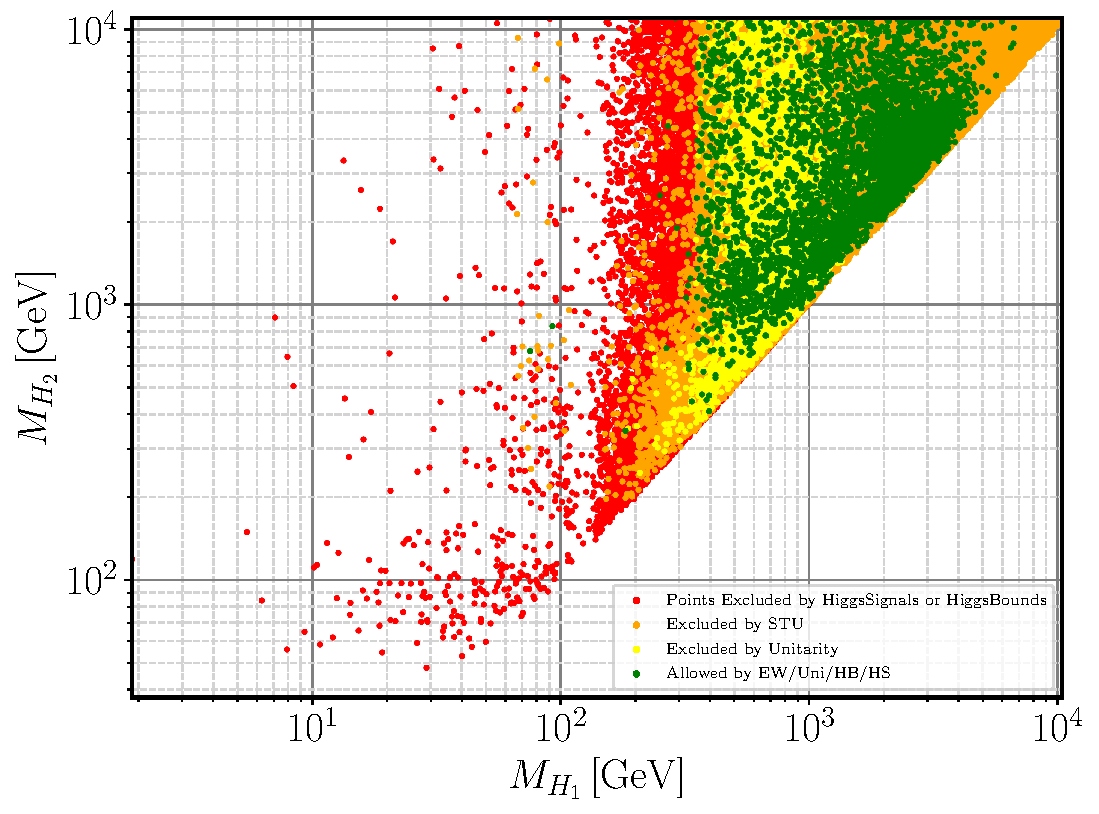
\includegraphics[width=.49\textwidth]{/3HDM/H1_H2.pdf}
	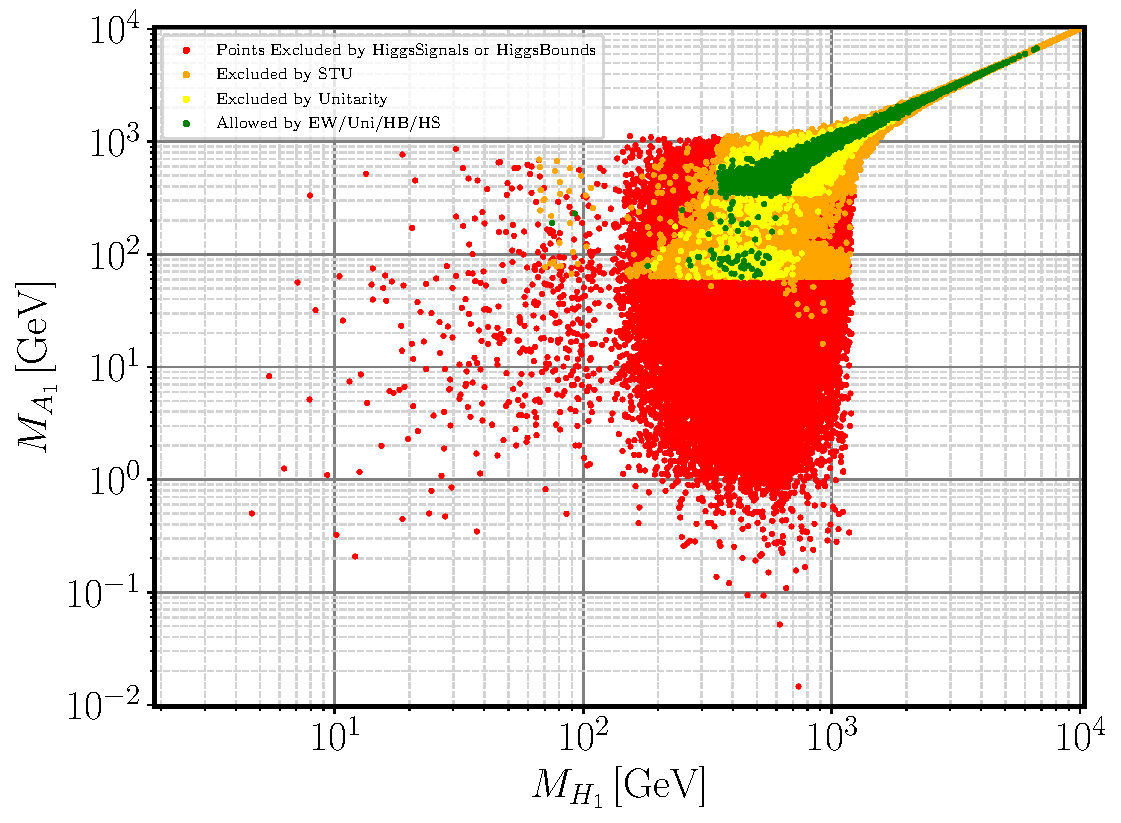
\includegraphics[width=.49\textwidth]{/3HDM/H1_A1.pdf}
	\caption{Scatter plots of parameter space allowed under  several cuts imposed on the BGL-like 3HDM. Right we have the plot showing the masses of the two heavier CP-even scalars $H_2$ and $H_1$ while in the right we show the relation between the lightest (non SM Higgs) of the CP-even and pseudoscalar particles. Red points failed HS and HB tests; yellow points violate unitarity constraints; orange points only fail electroweak precision constraints, and green ones satisfy all restrictions.}
	\label{fig:H1_A1_Plots}
\end{figure}	

\begin{figure}[H]
	\centering
	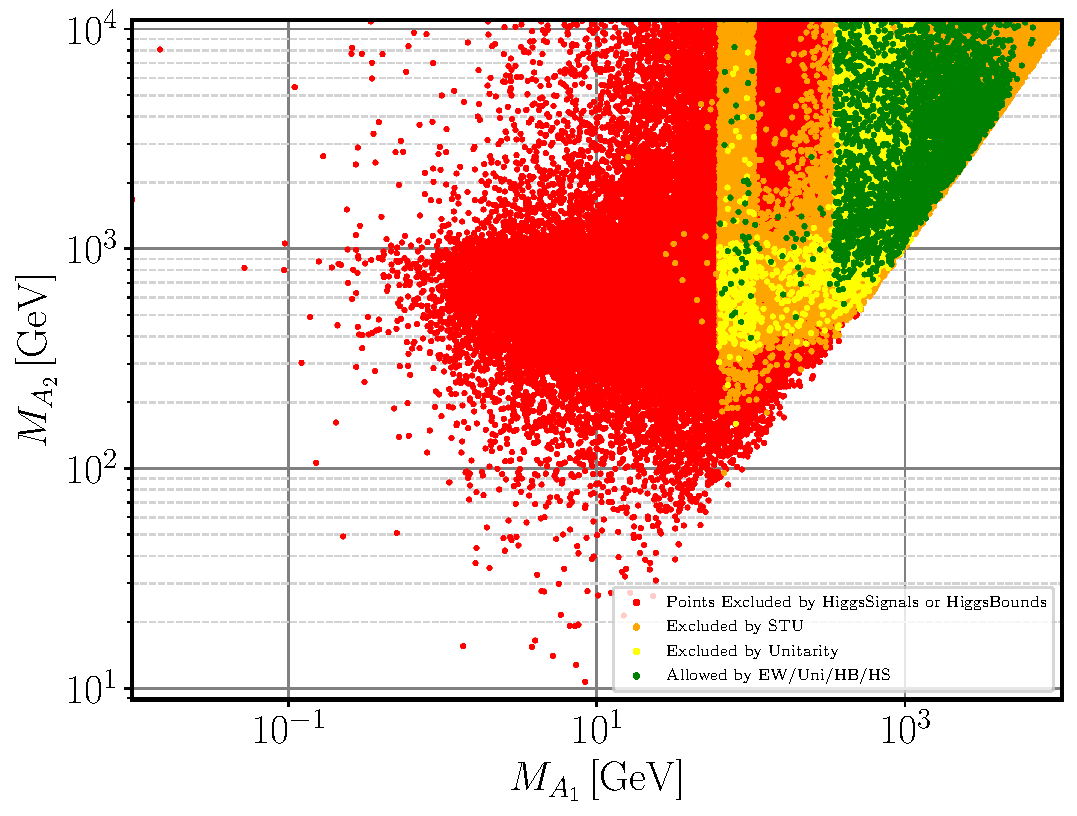
\includegraphics[width=.49\textwidth]{/3HDM/A1_A2.pdf}
	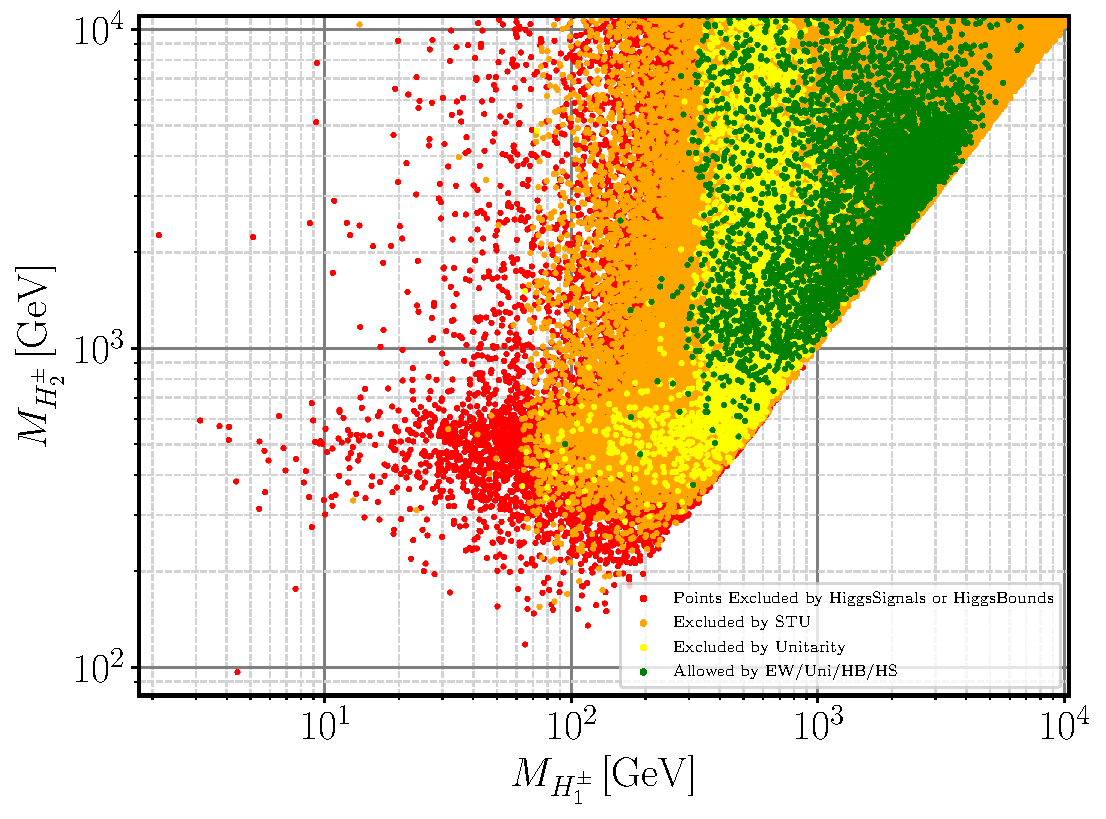
\includegraphics[width=.49\textwidth]{/3HDM/Hc1_Hc2.pdf}
	\caption{}
	\label{fig:Other_H_plots}
	\caption{Here we can see the remaining CP-odd scalars and how they are excluded under several cuts. Right we have the pseudoscalar masses $A_1$ and $A_2$ while in the left side we have the CP- odd charged Higgs states $H_1^\pm$ and $H_2^\pm$. Red points failed HS and HB tests; yellow points violate unitarity constraints; orange points only fail electroweak precision constraints, and green ones satisfy all restrictions.}
\end{figure}	

We can see that there a mass ordering between the scalar states, this is a automatic feature of SPheno that ensures a growing order of scalar masses. This change does not have any real physical significance but it leaves our graphs with a linear cut where $m_i = m_j$. 
%
We also omit showing the precise EW ellipsoids seeing their cuts are already shown in these figures. { \color{red} should I show this? } 

{ \color{red} why do pseudo scalar masses tend to funnel? } 

{ \color{red} what can I saw about the bottom graphics    } 

Note that, by requiring that we have a SM-like Higgs boson, naturally imposes conditions upon the couplings of the heavier (or lighter) CP-even scalar states to the Gauge bosons, and seeing that the harshest condition on most scalar sectors is the di-Z production we then have that due to the alignment limit imposed the majority of the scalar sector is allowed. 

We can also see that unless the signal coming from the pseudoscalar masses is masked by the Higgs SM signal or the pseudoscalar is heavy (in the TeV region) that it poses a harsh cut on the parameter space.

 { \color{red} Why then are the pseudoscalars so constricted. }   


\subsection{Flavour results}

After being finished with the analysis for the scalar sector we can see exactly what the flavour observables can tell us. We define the exclusion of a point based flavour observables as it being over a $2 \sigma$ bound for that QFV.  




\begin{figure}[H]
	\centering
	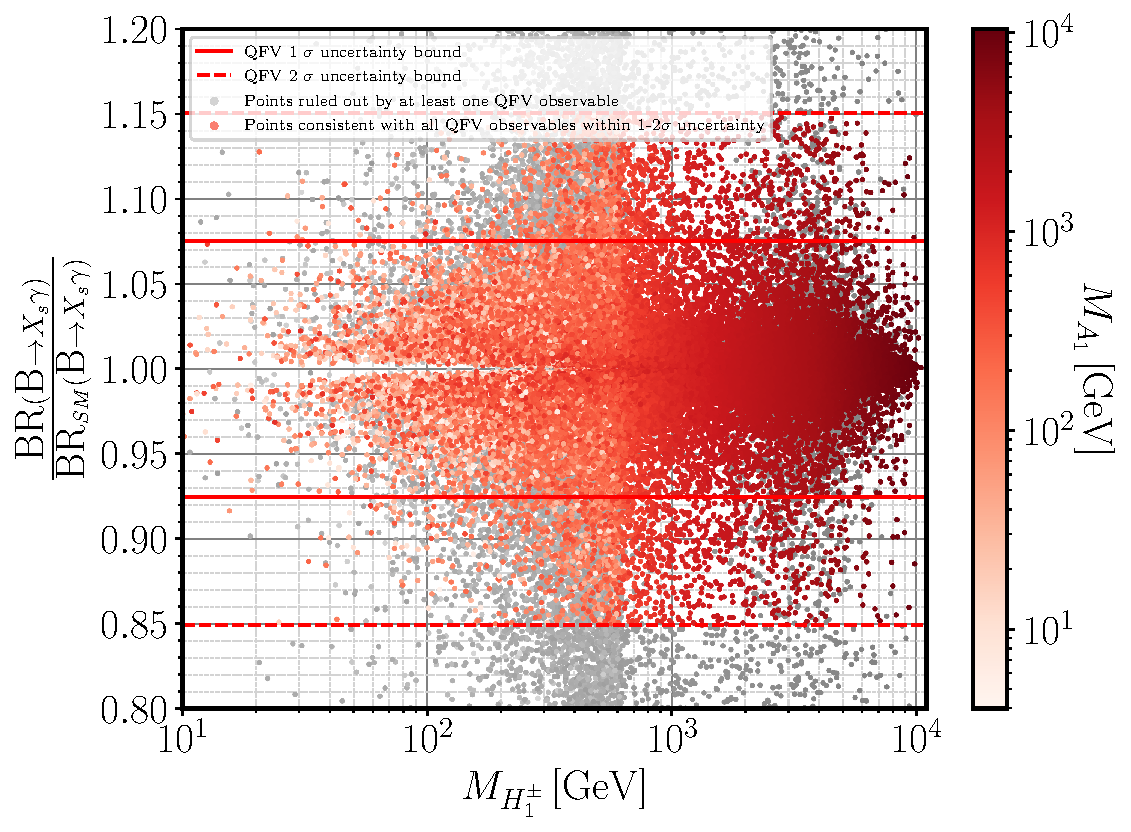
\includegraphics[width=.75\textwidth]{/3HDM/Xsgamma_Hc1_A1.pdf}
	\caption{}
	\label{fig:STU_2}
\end{figure}	

\subsubsection{Fine-Tuning}


\subsection{Flavour and Scalar cuts }

Having shown that there are no instances of heavy fine tuning in our model. 

\begin{figure}[H]
	\centering
	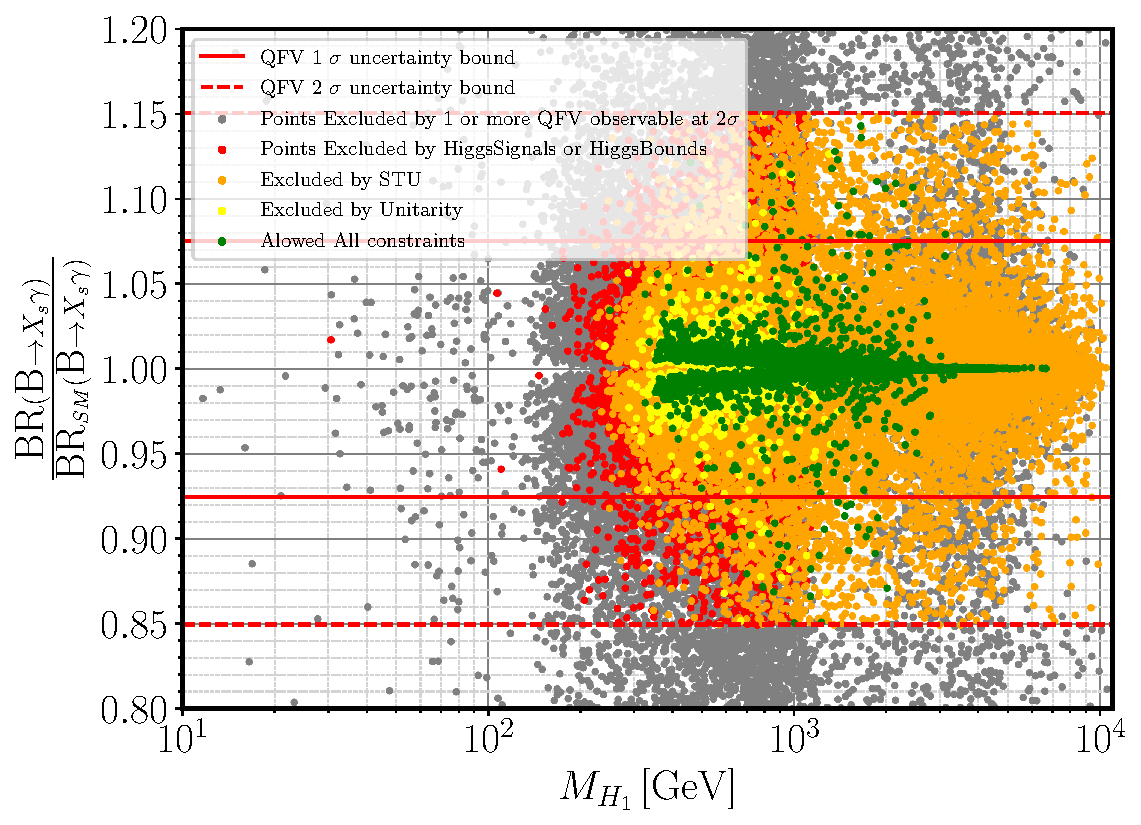
\includegraphics[width=.49\textwidth]{/3HDM/XsGamma_H1.pdf}
	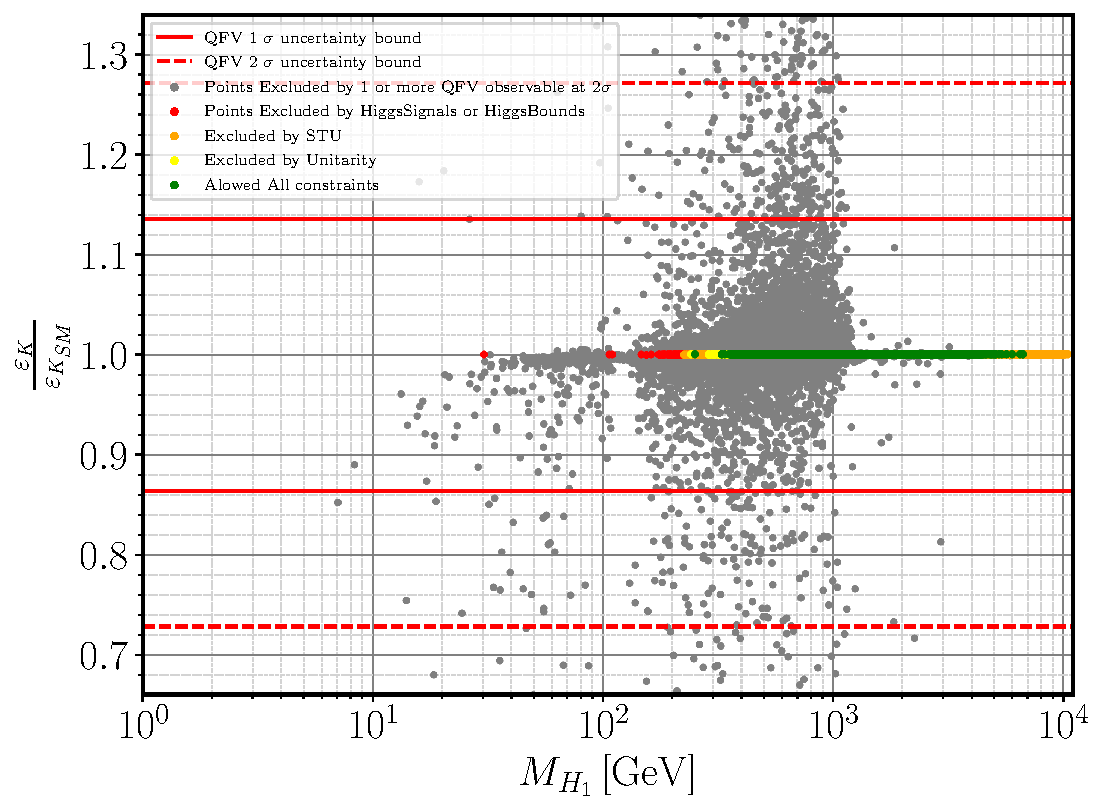
\includegraphics[width=.49\textwidth]{/3HDM/Eps_K_H1.pdf}
	\caption{Scatter plots of parameter space allowed under  several cuts imposed on the BGL-like 3HDM. Right we have the plot showing the masses of the two heavier CP-even scalars $H_2$ and $H_1$ while in the right we show the relation between the lightest
(non-h) of the CP-even and pseudoscalar particles. Red points failed HS and HB tests; yellow points violate unitarity constraints; orange points only fail electroweak precision constraints, and green ones satisfy all restrictions.}
	\label{fig:PT_plots_H1}
\end{figure}	

\begin{figure}[H]
	\centering
	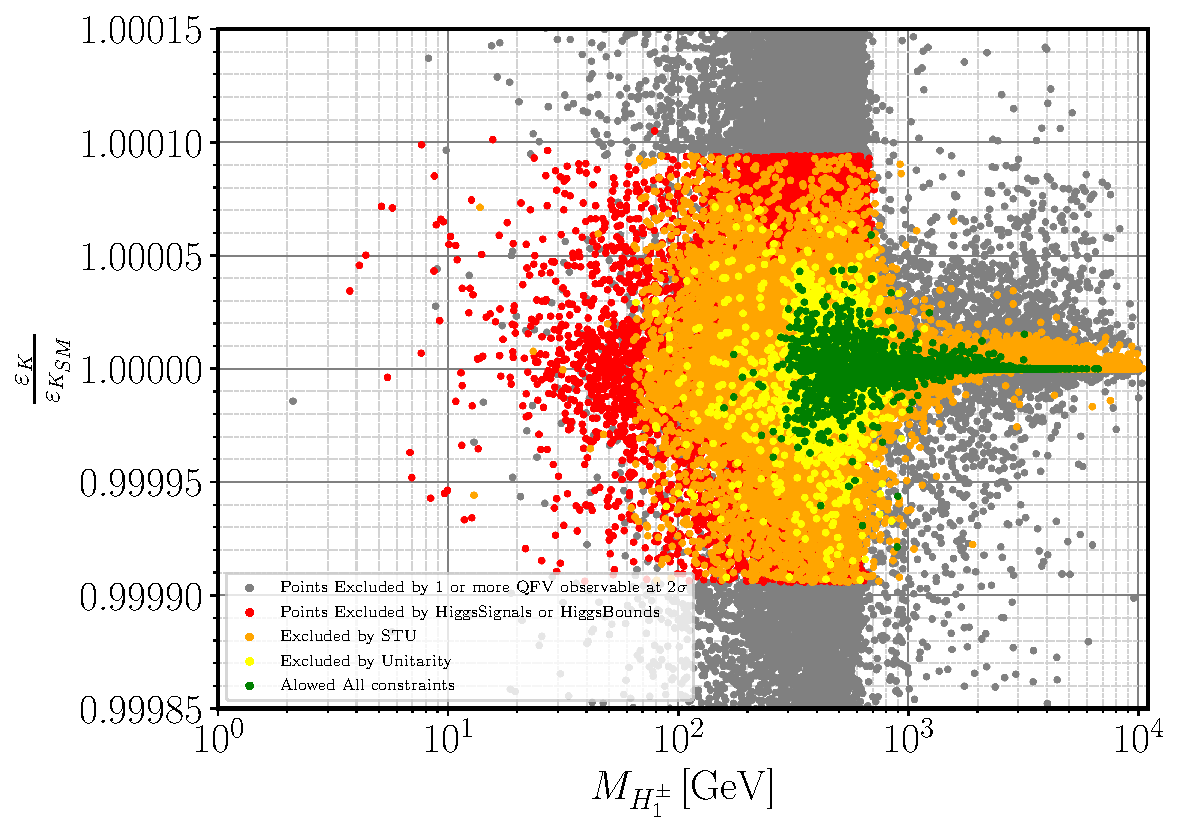
\includegraphics[width=.75\textwidth]{/3HDM/Eps_K_Hc1_Thighter_Centered.pdf}
	\caption{}
	\label{fig:STU_3}
\end{figure}	




